\section{Application specification}
\label{sec:app:specification}

To give a short overview to the environment we use the four nodes of our microcontroller network are shown in figure \ref{fig:app:specification:node_overview} \nameref{fig:app:specification:node_overview} 
and outline the functionalities provided by the single nodes useful for our application level.\\

\begin{figure}[t]
 \centering
 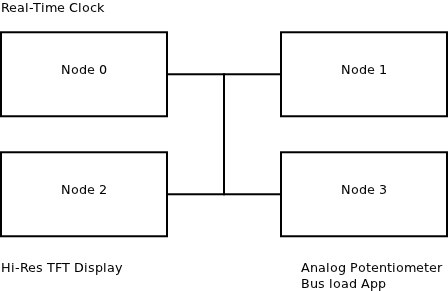
\includegraphics[scale=0.5]{../images/node_overview.png}
 % node_tasks.png: 448x291 pixel, 72dpi, 15.80x10.27 cm, bb=
 \caption{capabilities of nodes}
 \label{fig:app:specification:node_overview}
\end{figure}

\subsection{Node 0}
\label{sec:app:specification:node0}

\subsection{Node 1}
\label{sec:app:specification:node1}

\subsection{Node 2}
\label{sec:app:specification:node2}

Node 2 is used to provide monitoring services via the lcd. For this purpose no filtering of messages is provided by the protocol.
All messages crossing the bus are stored and evaluated to certain properties such as

\begin{enumerate}
 \item the drifts of the certain clocks
 \item message loss rates
\end{enumerate}

and can be visualized via the lcd as pure text or as chart.\\

A sketch how the visualization could look is given in figure \ref{fig:app:specification:node2} \nameref{fig:app:specification:node2}.

\begin{figure}[t]
 \centering
 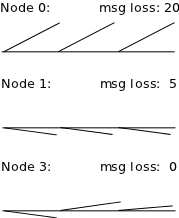
\includegraphics[scale=0.8]{../images/app_visu_sketch.png}
 % node_tasks.png: 448x291 pixel, 72dpi, 15.80x10.27 cm, bb=
 \caption{sketch of visualization}
 \label{fig:app:specification:node2}
\end{figure}


\subsection{Node 3}
\label{sec:app:specification:node3}

% 
% 
% \subsection{Bus load app}
% \label{app_specification:bus_load}
% Has the benefit of user adjustable provocation load rates for 
% further testing
% 
% The load app will provide different bus injection methods
% \subsubsection{Fault Injection via Buttons}
% Is the ability to inject faulty transmissions into the bus by pressing
% a button to check the fail-safetyness of the bus and the protocol.
% 
% This is meant to be the pendant of an electro magnetic disturbance
% injected into the bus cable and should be detected through the
% CRC sums by the receiver.
% 
% \subsubsection{Overload Simulation via Buttons}
% Is the ability to inject heavy bus load by pressing a button to
% check the accessibility of the bus if the bus is busy. 
% See also: \ref{app_specification:drift_rates} \nameref{app_specification:drift_rates}
% 
% \subsection{Drift rates}
% \label{app_specification:drift_rates}
% The main target of our application is to show drifts of the synchronous 
% clocks in our network. 
% 
% That means that we are measuring:
% \begin{itemize}
%  \item The ability of the nodes to synchronize the clocks via the bus 
% while it is under load due to the bus load application
%  \item The drifts between the clocks before synchronizing
% \end{itemize}
% 
% \subsection{Visualization of Drift Rates via LCD}
% The visualization is planned via a difference bar charts on the 
% LCD display of the uC board.
% 
% \subsection{Debugging and Monitoring features via PC}
% The ability to debug through the PC is one of the first 
% feature most developers are looking for. Therefore, it is an
% nice to have feature for us to engineer. 
% 
% This method could only unfold its full advantage in an emerging 
% developer version where the bus will be used in action.




% The application is ment to run distributed 
% as shown in figure \ref{fig:node_task_assignment} \nameref{fig:node_task_assignment}
% 
% 
% \subsection{Node2}
% Node2 will take over the task of visualization described in
% \ref{app_specification:drift_rates} \nameref{app_specification:drift_rates}
% 
% \subsection{Node3}
% Node0 will take over the task of the bus load application
% \ref{app_specification:bus_load} \nameref{app_specification:bus_load}